\section{Methodology }\label{sec:meth}
In this project, we consider the sections in the algorithm that can be parallelized, 
write kernels for each of them and offload them to be executed on GPU. 
The sections that can be parallelized are explained below.
1. Image pyramid:
We use fixed size (20x20) for each feature. But the face in the image can be of any scale. 
To make the face detection scale  invariant, we use pyramid of images that contains upscale and
downscale versions of the original image. Since each pixel can be processed separately, 
we intend to produce image pyramid on GPU. Example of an image pyramid is shown in Figure~\ref{fig:scale}.

\begin{figure}[h]
  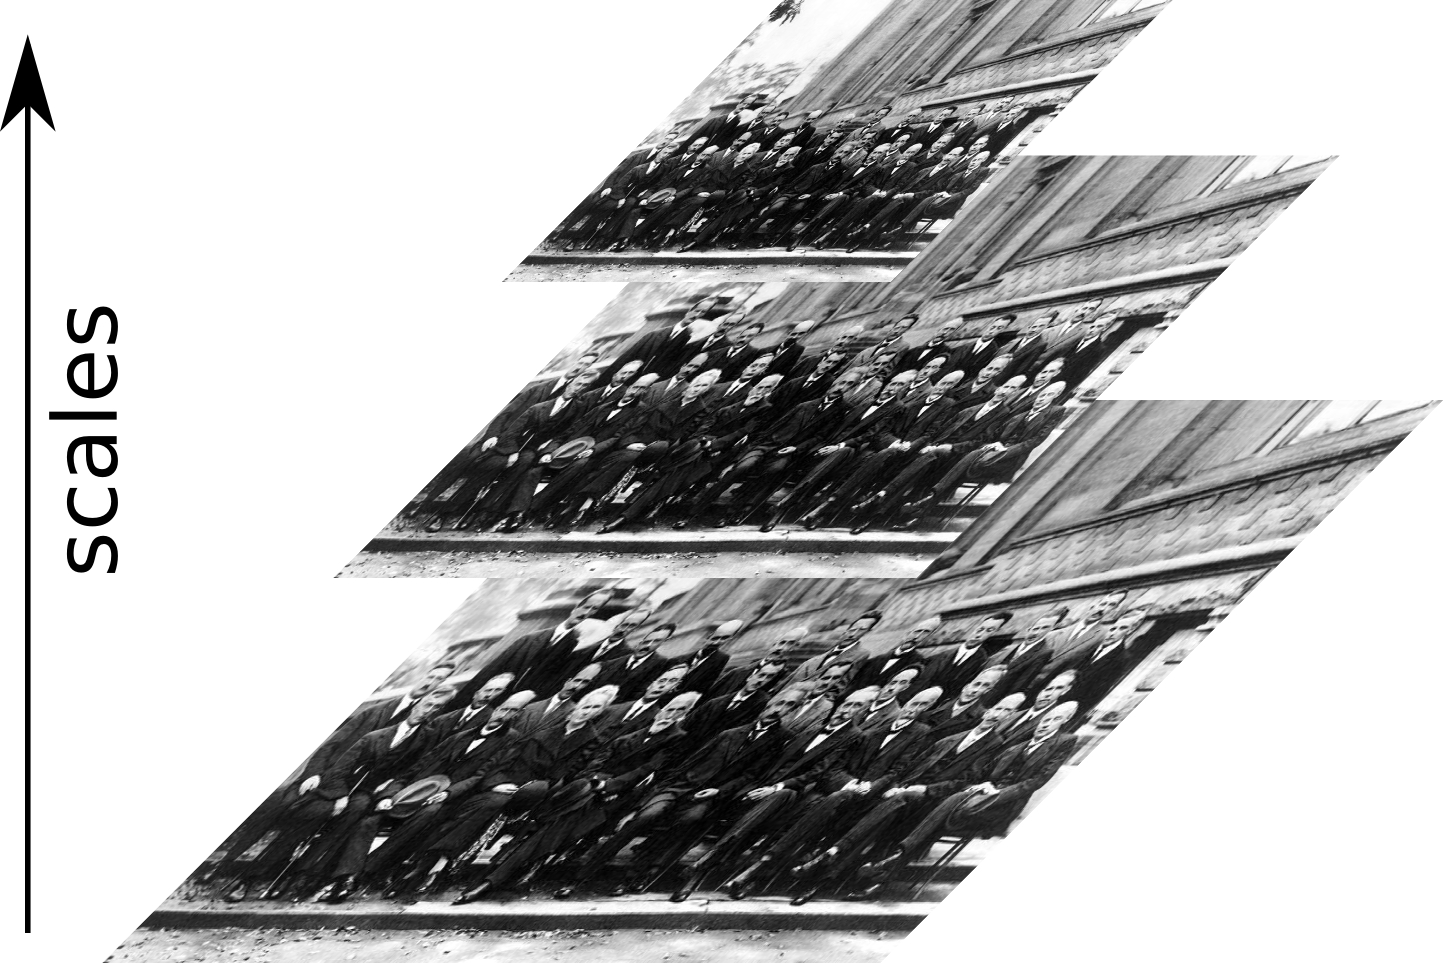
\includegraphics[width=0.45\linewidth]{figs/scale.jpg}
  \caption{Image Pyramid \textnormal{\small }  }
  \label{fig:scale}
\end{figure}

2. Integral image calculation:
Integral image calculation is essentially 2-dimensional inclusive scan. Since we have already done 
1-dimensional prefix scan on GPU and seen the benefits, we intend to determine integral image on 
similar lines.
To avoid data dependency of image integral calculation, we adopt the algorithm of first 
row integral and then column integral calculation.

3. Scan window processing:
Since each 20x20 image sub-window has to pass through all the features, each thread in the GPU 
can perform parallely on a sub-window. But the design of cascade classifier is such that after 
each stage the doubtless non-face scan sub-windows are eliminated as much as possible. Hence we 
want to consider each stage separately and sequentially, may be execute each stage as a different kernel.


